\documentclass[aspectratio=169,11pt]{beamer}

\usepackage[T1]{fontenc}
\usepackage{lmodern}
\usepackage{tikz}
\usetikzlibrary{positioning,arrows.meta,calc,fit,shapes.geometric}
\usepackage{booktabs}

% ---------- palette ----------
\definecolor{ink}{HTML}{14213D}
\definecolor{paper}{HTML}{FBFBF8}
\definecolor{accent}{HTML}{E07A1F}
\definecolor{blue}{HTML}{2E6F95}
\definecolor{greyb}{HTML}{E4E6EA}
\definecolor{muted}{HTML}{4A5568}

% ---------- beamer look ----------
\setbeamercolor{normal text}{fg=ink,bg=paper}
\setbeamercolor{background canvas}{bg=paper}
\setbeamercolor{title}{fg=ink}
\setbeamercolor{frametitle}{fg=ink,bg=paper}
\setbeamercolor{structure}{fg=blue}
\setbeamercolor{itemize item}{fg=accent}
\setbeamercolor{block title}{fg=paper,bg=blue}
\setbeamercolor{block body}{fg=ink,bg=greyb}
\setbeamerfont{frametitle}{size=\LARGE,series=\bfseries}
\setbeamerfont{title}{size=\LARGE,series=\bfseries}
\setbeamerfont{block title}{size=\normalsize,series=\bfseries}
\setbeamertemplate{navigation symbols}{}
\setbeamertemplate{footline}[frame number]
\setbeamertemplate{itemize items}[circle]
\setbeamersize{text margin left=12mm,text margin right=12mm}

\title{Matrix-Multiply Accelerator on a RISC-V SoC}
\subtitle{4$\times$4, 6$\times$6 and 8$\times$8 systolic arrays on the Boolean board}
\author{Course project}
\date{}

% ---------- reusable TikZ styles ----------
\tikzset{
  pe/.style={draw=ink, line width=0.8pt, fill=accent!30, rounded corners=2pt,
             minimum size=9mm, font=\small},
  box/.style={draw=ink, line width=0.8pt, rounded corners=4pt, align=center,
              minimum height=12mm, inner sep=4pt, font=\small},
  grey/.style={box, fill=greyb},
  orange/.style={box, fill=accent},
  bluebox/.style={box, fill=blue, text=paper},
  link/.style={-{Stealth[length=2mm]}, line width=0.9pt, ink},
  datalink/.style={-{Stealth[length=2mm]}, line width=1.4pt, blue},
  resultlink/.style={-{Stealth[length=2mm]}, line width=1.4pt, accent}
}

\begin{document}

% ==================================================================
\begin{frame}[plain]
  \vfill
  \begin{tikzpicture}[remember picture,overlay]
    % decorative systolic-grid backdrop
    \foreach \i in {0,...,5} \foreach \j in {0,...,8} {
      \fill[accent!18] ($(current page.south east)+(-\j*0.42-0.5,\i*0.42+0.4)$) rectangle +(0.32,0.32);
    }
  \end{tikzpicture}
  \begin{minipage}{0.62\textwidth}
    {\Large\bfseries\color{ink} Matrix-Multiply Accelerator\\on a RISC-V SoC\par}
    \vspace{4mm}
    {\large\color{muted} 4$\times$4, 6$\times$6 and 8$\times$8 systolic arrays\\running on the Boolean board (Xilinx XC7S50)\par}
    \vspace{8mm}
    {\color{blue}\rule{40mm}{1.2pt}}\\[3mm]
    {\small\color{muted} Course project presentation}
  \end{minipage}
  \vfill
\end{frame}

% ==================================================================
\begin{frame}{A systolic array multiplies matrices in a grid}
  \begin{columns}[T,onlytextwidth]
    \begin{column}{0.56\textwidth}
      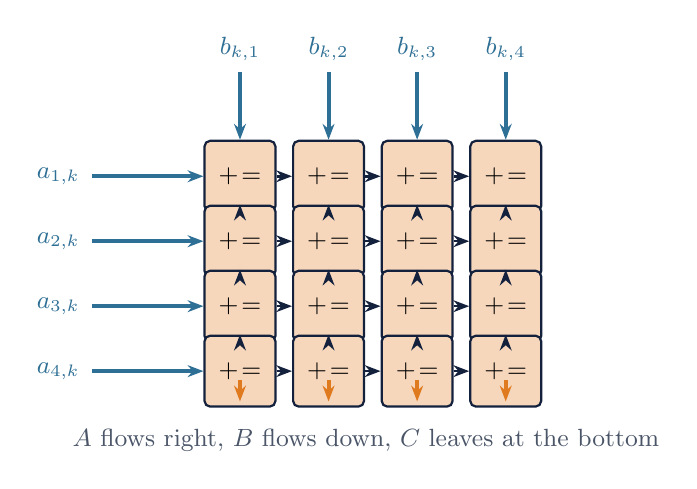
\begin{tikzpicture}[x=0.75cm,y=0.55cm]
        % PE grid: 4x4, PE (i,j) at (j*1.5, -i*1.5)
        \foreach \i in {1,...,4} \foreach \j in {1,...,4} {
          \node[pe] (pe\i\j) at (\j*1.5,-\i*1.5) {$+\!=$};
        }
        % A streams in from the left, one per row, moving right
        \foreach \i in {1,...,4} {
          \draw[datalink] (-1.0,-\i*1.5) -- (pe\i1.west);
          \node[left,font=\small,blue] at (-1.05,-\i*1.5) {$a_{\i,k}$};
        }
        % B streams in from the top, one per column, moving down
        \foreach \j in {1,...,4} {
          \draw[datalink] (\j*1.5,0.9) -- (pe1\j.north);
          \node[above,font=\small,blue] at (\j*1.5,0.95) {$b_{k,\j}$};
        }
        % forwarding between neighbours
        \foreach \i in {1,...,4} \foreach \j in {1,...,3} {
          \draw[link] (pe\i\j.east) -- (pe\i\the\numexpr\j+1\relax.west);
        }
        \foreach \i in {1,...,3} \foreach \j in {1,...,4} {
          \draw[link] (pe\i\j.south) -- (pe\the\numexpr\i+1\relax\j.north);
        }
        % results leave at the bottom
        \foreach \j in {1,...,4} {
          \draw[resultlink] (\j*1.5,-6.2) -- (\j*1.5,-6.7);
        }
        \node[font=\small,muted,anchor=west] at (-1.5,-7.6) {$A$ flows right, $B$ flows down, $C$ leaves at the bottom};
      \end{tikzpicture}
    \end{column}
    \begin{column}{0.40\textwidth}
      \begin{itemize}
        \item One multiply-add per PE per cycle
        \item Each PE owns one element of $C$ (output-stationary)
        \item Array size is a parameter: $N\times N$ PEs
        \item Operands int16, accumulators 48-bit, low 32 bits to $C$
      \end{itemize}
    \end{column}
  \end{columns}
\end{frame}

% ==================================================================
\begin{frame}{Two bus ports connect the accelerator}
  \begin{center}
  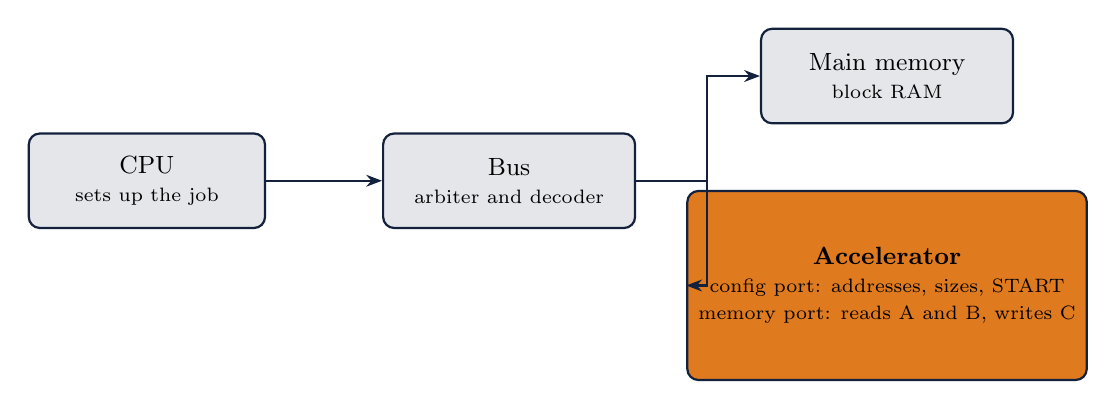
\begin{tikzpicture}[x=1cm,y=0.7cm]
    \node[grey,minimum width=30mm] (cpu) at (0,0) {CPU\\[-1pt]{\scriptsize sets up the job}};
    \node[grey,minimum width=32mm] (bus) at (4.6,0) {Bus\\[-1pt]{\scriptsize arbiter and decoder}};
    \node[grey,minimum width=32mm,minimum height=12mm] (mem) at (9.4,1.9) {Main memory\\[-1pt]{\scriptsize block RAM}};
    \node[orange,minimum width=40mm,minimum height=24mm] (acc) at (9.4,-1.9) {\textbf{Accelerator}\\[-1pt]{\scriptsize config port: addresses, sizes, START}\\[-1pt]{\scriptsize memory port: reads A and B, writes C}};

    \draw[link] (cpu) -- (bus);
    \draw[link] (bus.east) -- ++(0.9,0) |- (mem.west);
    \draw[link] (bus.east) -- ++(0.9,0) |- (acc.west);
  \end{tikzpicture}
  \end{center}
  \vspace{1mm}
  {\small The CPU writes the job's addresses and sizes and presses START. The accelerator then fetches its own inputs and writes its results back.}
\end{frame}

% ==================================================================
\begin{frame}{The board has no external RAM}
  \begin{columns}[T,onlytextwidth]
    \begin{column}{0.58\textwidth}
      \textbf{One $256\times256$ int32 matrix is 256\,KB}
      \vspace{2mm}
      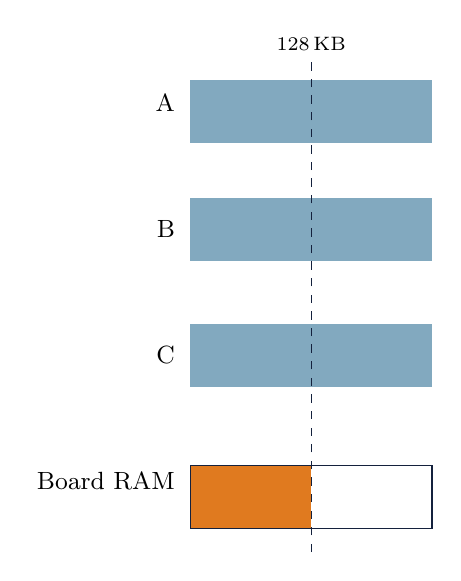
\begin{tikzpicture}[x=0.012cm,y=1cm]
        % 1 unit = 1 KB horizontally
        \node[anchor=east,font=\small] at (-6,0.5) {A};
        \fill[blue!60] (0,0) rectangle (256,0.8);
        \node[anchor=east,font=\small] at (-6,-1.1) {B};
        \fill[blue!60] (0,-1.5) rectangle (256,-0.7);
        \node[anchor=east,font=\small] at (-6,-2.7) {C};
        \fill[blue!60] (0,-3.1) rectangle (256,-2.3);
        \node[anchor=east,font=\small] at (-6,-4.3) {Board RAM};
        \fill[accent] (0,-4.9) rectangle (128,-4.1);
        \draw[ink,line width=0.6pt] (0,-4.9) rectangle (256,-4.1);
        \draw[dashed,ink] (128,-5.2) -- (128,1.1);
        \node[font=\scriptsize,anchor=south] at (128,1.05) {128\,KB};
      \end{tikzpicture}
      \vspace{3mm}
      \begin{itemize}
        \item Three full matrices (768\,KB) cannot fit on-chip
        \item So the PC keeps the matrices and sends 64$\times$64 blocks
      \end{itemize}
    \end{column}
    \begin{column}{0.38\textwidth}
      \begin{block}{How the data moves}
        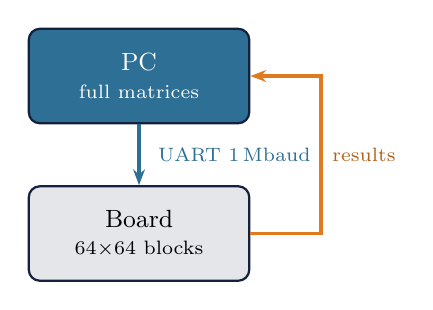
\begin{tikzpicture}[x=1cm,y=1cm]
          \node[bluebox,minimum width=28mm] (pc) at (0,0) {PC\\[-1pt]{\scriptsize full matrices}};
          \node[grey,minimum width=28mm] (fw) at (0,-2.0) {Board\\[-1pt]{\scriptsize 64$\times$64 blocks}};
          \draw[datalink] (pc) -- node[right,font=\scriptsize,blue] {\hspace{1mm}UART 1\,Mbaud} (fw);
          \draw[resultlink] (fw.east) -- ++(0.9,0) |- node[near start,right,font=\scriptsize,accent!80!black] {results} (pc.east);
        \end{tikzpicture}
      \end{block}
    \end{column}
  \end{columns}
\end{frame}

% ==================================================================
\begin{frame}{SoC overview: existing parts and what we added}
  \begin{center}
  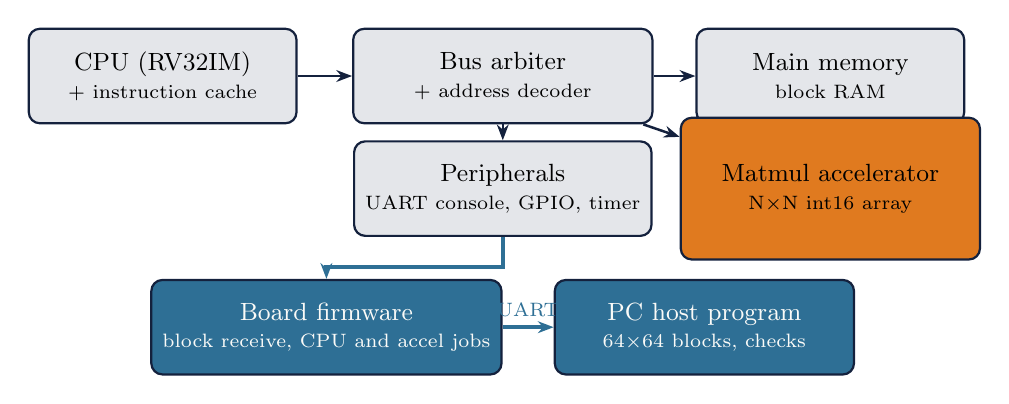
\begin{tikzpicture}[x=0.8cm,y=0.55cm]
    \node[grey,minimum width=34mm] (cpu) at (0,2.4) {CPU (RV32IM)\\[-1pt]{\scriptsize + instruction cache}};
    \node[grey,minimum width=38mm] (bus) at (5.4,2.4) {Bus arbiter\\[-1pt]{\scriptsize + address decoder}};
    \node[grey,minimum width=34mm] (mem) at (10.6,2.4) {Main memory\\[-1pt]{\scriptsize block RAM}};

    \node[grey,minimum width=34mm] (per) at (5.4,-0.2) {Peripherals\\[-1pt]{\scriptsize UART console, GPIO, timer}};
    \node[orange,minimum width=38mm,minimum height=18mm] (acc) at (10.6,-0.2) {Matmul accelerator\\[-1pt]{\scriptsize N$\times$N int16 array}};

    \node[bluebox,minimum width=38mm] (fw) at (2.6,-3.4) {Board firmware\\[-1pt]{\scriptsize block receive, CPU and accel jobs}};
    \node[bluebox,minimum width=38mm] (pc) at (8.6,-3.4) {PC host program\\[-1pt]{\scriptsize 64$\times$64 blocks, checks}};

    \draw[link] (cpu) -- (bus);
    \draw[link] (bus) -- (mem);
    \draw[link] (bus) -- (per);
    \draw[link] (bus) -- (acc);
    \draw[datalink] (per.south) -- ++(0,-0.7) -| (fw.north);
    \draw[datalink] (fw.east) -- node[above,font=\scriptsize,blue] {UART} (pc.west);
  \end{tikzpicture}
  \end{center}
  \vspace{-2mm}
  
\begin{tikzpicture}[x=1cm,y=1cm]
    \node[grey,minimum width=6mm,minimum height=4mm] (a) at (0,0) {};
    \node[anchor=west,font=\small] at (0.5,0) {existing};
    \node[orange,minimum width=6mm,minimum height=4mm] (b) at (3.2,0) {};
    \node[anchor=west,font=\small] at (3.7,0) {added: accelerator};
    \node[bluebox,minimum width=6mm,minimum height=4mm] (c) at (7.2,0) {};
    \node[anchor=west,font=\small] at (7.7,0) {added: PC link and firmware};
  \end{tikzpicture}
\end{frame}

% ==================================================================
\begin{frame}{Results: speed-up over the CPU}
  \begin{center}
  \begin{tabular}{l ccc}
    \toprule
    & \multicolumn{3}{c}{Matrix size} \\
    \cmidrule(lr){2-4}
    PE array & $128\times128$ & $256\times256$ & $512\times512$ \\
    \midrule
    $4\times4$ (16 PEs) & 32.5$\times$ / 1.85$\times$ & 32.5$\times$ / 2.25$\times$ & 32.5$\times$ / 2.50$\times$ \\
    $6\times6$ (36 PEs) & 52.9$\times$ / 1.98$\times$ & 52.9$\times$ / 2.31$\times$ & 52.9$\times$ / 2.52$\times$ \\
    $8\times8$ (64 PEs) & 77.3$\times$ / 1.95$\times$ & 77.3$\times$ / 2.26$\times$ & 77.3$\times$ / 2.53$\times$ \\
    \bottomrule
  \end{tabular}
  \end{center}
  \vspace{4mm}
  \begin{columns}[T,onlytextwidth]
    \begin{column}{0.48\textwidth}
      \begin{block}{Left number: compute only}
        CPU cycles $\div$ accelerator cycles
      \end{block}
    \end{column}
    \begin{column}{0.48\textwidth}
      \begin{block}{Right number: end-to-end}
        includes UART transfers, as a user sees it
      \end{block}
    \end{column}
  \end{columns}
  \vspace{2mm}
  {\footnotesize Board runs at 25\,MHz. Every result checked against a PC reference.}
\end{frame}

% ==================================================================
\begin{frame}{Limitations and future work}
  \begin{columns}[T,onlytextwidth]
    \begin{column}{0.48\textwidth}
      \begin{block}{Limitations}
        \begin{itemize}
          \item The 32-bit bus: loads are about 80\% of accelerator cycles
          \item UART transfers cap end-to-end speed-up near 2.5$\times$
          \item Board RAM caps the block size
          \item 10$\times$10 array failed the memory routing check
        \end{itemize}
      \end{block}
    \end{column}
    \begin{column}{0.48\textwidth}
      \begin{block}{Future work}
        \begin{itemize}
          \item Pack two int16 values per memory word
          \item Rectangular blocks (for example 128$\times$64)
          \item Large sizes on the Arty A7 with DDR3
          \item A wider memory path or DMA
        \end{itemize}
      \end{block}
    \end{column}
  \end{columns}
\end{frame}

% ==================================================================
\begin{frame}{AI usage declaration}
  Claude (Anthropic) was used to help understand and implement the Verilog for the accelerator and SoC changes, the C test and PC host software, and the Vivado and board build scripts.
  \vspace{3mm}

  The author made the design decisions, reviewed all generated code, ran the simulations and board runs, and produced the results in this presentation.
\end{frame}

\end{document}
